\documentclass{article}
\usepackage{graphicx}
\usepackage{hyperref}
\usepackage[a4paper, margin=1.25in]{geometry}
\usepackage{breakcites}
\usepackage{subcaption}
\usepackage{float}
\usepackage{textcomp}
\usepackage{amsmath}
\usepackage{textgreek}
\usepackage{authblk}
\usepackage{rotating}
\usepackage{booktabs}
\usepackage{longtable}
\usepackage{pdflscape}
\usepackage{lineno}
\usepackage[
  style=numeric,
  citestyle=numeric-comp,
  backend=biber,
  doi=true,
  natbib=true,
  sorting=none
]{biblatex}

\addbibresource{TextDataClimateShocks.bib}

\begin{document}

\title{Heatwaves Exacerbate Inequalities in Mental Health}

%\author[1, *]{Matthew Cooper}
%\author[]{Jeremiah Osborne-Gowey}
%\author[]{Zheng Liu}
%\author[]{Jie Liu}
%\author[]{Portia Adade Williams}
%\author[]{Aaron Schwartz}
%\author[]{Patrick Baylis}

%\affil[1]{T.H. Chan School of Public Health, Harvard University}
%\affil[*]{Corresponding Author: mcooper@hsph.harvard.edu}

\maketitle

\begin{abstract}
Weather can affect people’s mood and well-being. Traditional studies exploring the effects of weather on mental health require significant resource investment (e.g., time, funding, execution).  Continuous in situ data streams from social media, newspapers, and other big data sources offer an opportunity to examine how people perceive and respond to environmental conditions. Recent work demonstrates that prevailing weather conditions can affect people’s sentiment as expressed on Twitter and other social media.  Studies to date however, have modeled the weather as having the same effect on sentiment across all locations and individuals (i.e., in aggregate).  In this study, we explore how weather affects individual expressed sentiment (via Twitter) across different weather gradients and locations. We analyzed the sentiment from a quarter of a billion geolocated Tweets from 2009 to 2019, using multiple measures of sentiment, overlaid with data about prevailing weather conditions, as well as local land cover, income levels, and demographic characteristics in the vicinity of Twitter users.  We find that weather affects people differently across a range of incomes, with people in higher income brackets generally happier with increasing temperature, while people in lower income brackets are less happy with increasing temperature.  This project extends existing research about the relationship between temperature and mood (sentiment) by examining how varying climatic conditions across different geographies and socio-economic groups are correlated with expressed sentiment. This project brings new insights into how humans perceive and respond to environmental shocks, with important implications for economics, policy and adaptation and resilience planning.

\end{abstract}

Keywords: Text Data, Environmental Shocks, Social Media Mining, Sentiment Analysis, Topic Modeling, Social Media, Public Opinion, Perception, Sentiment, Media, News, Twitter, Climate Change, Science Communication, Policy, Planning, Methods, Text Mining, Natural Language Processing, NLP, Latent Dirichlet Allocation, LDA, Political Ecology, Politics, Resilience, Adaptation

    
%Cite this new paper: https://doi.org/10.1016/S2542-5196(20)30251-5

\section{Introduction}

% Organize as follows:

% Heatwaves are known to worsen mental health
% AND mental health is strongly associated with income
% AND wealthier better able to cope with heatwaves 
% BUT we know little about the interaction between heatwaves, mental health and income
% THEREFORE: we did this really novel study.

This work builds on existing work by \citep{baylis_weather_2018}. 

%Intro Paragraph
Research has demonstrated strong linkages between ambient environmental conditions and mental health, with extreme temperatures more frequently associated with poorer overall mental health. Mental health is strongly associated with income with people in lower income levels frequently experiencing higher stress levels and less capable of finding help for coping with these stresses. Additionally, results from research on how people cope with environmental temperature extremes indicate that wealthier are better able to cope with heatwaves. Furthermore, previous studies examining relationships between environmental extremes and health sometimes aggregate data at scales too coarse to examine whether income may be an ameliorating factor. Yet we know relatively little about the interaction between temperature, mental health and income. This research examines the interactions between these three using relatively fine-scale, publicly available data. This study expands on existing temperature and sentiment - one measure of mental health - research by examining finer-scale data and incorporating income data to examine correlations between extreme temperatures and sentiment.

Human moods and mental states are important aspects of overall well-being and can be influenced by ambient and persistent environmental conditions. Climate change is accelerating the rate and variability around meteorological norms like the timing, magnitude, intensity and duration of precipitation events and air temperature minima and maxima \href{https://www.ipcc.ch/site/assets/uploads/2018/03/SREX-Chap3_FINAL-1.pdf}{(link)}. Previous work \citep{baylis_weather_2018} indicate important linkages between human mood and meterological conditions. Previous analyses of the effects of weather on mood (as expressed in sentiment of text-based message), however, were constructed at the aggregated city/day level and did not account for differences in socio-economic status which may affect access to resources (e.g., air conditioning) that can offset the effects of exposure to meteorological conditions. Here, we build on these previous studies by examining the hourly effects of weather on human sentiment, an expression of mood, exploring geographic and economic heterogeneity at a finer-scale resolution than previous studies.  


\section{Background}
% Heatwaves are known to worsen mental health
https://doi.org/10.1016/j.puhe.2018.06.008 (review study - will have more to cite)
https://www.nature.com/articles/s41558-018-0222-x
https://ehp.niehs.nih.gov/doi/full/10.1289/ehp.11339

% AND mental health is strongly associated with income
https://jamanetwork.com/journals/jamapsychiatry/fullarticle/211213
https://doi.org/10.1002/9781118410868.wbehibs570
https://www.sciencedirect.com/science/article/abs/pii/S027795362030527X
https://www.sciencedirect.com/science/article/pii/S2468266717300117
https://doi.org/10.1016/S2468-2667(17)30011-7
https://link.springer.com/article/10.1007/s00127-017-1370-4

% AND wealthier better able to cope with heatwaves 
https://www.nature.com/articles/nclimate3253
https://www.sciencedirect.com/science/article/abs/pii/S0378778818321327

% BUT we know little about the interaction between heatwaves, mental health and income


% THEREFORE: we did this really novel study.

%OTHER LEFTOVER TEXT TO MAYBE BRING IN LATER



Meteorological conditions can impact human physical (cite) and emotional states (cite). Emotional states and well-being are associated with physiological functioning and mental acuity which can affect social relationships, workplace productivity (cite) and health risks (cite). People that are more reliant on livelihoods which require them to be outdoors (e.g., farming, agriculture, logging, etc.), living and working in places where they are exposed to environmental minima and maxima, or with prolonged exposure to ambient meteorological extremes are particularly vulnerable to changes in environmental exposure \citep{frimpong_heat_2017} and associated health risks (cite), with implications for workplace productivity and livelihoods \cite{kjellstrom_impact_2016}. For example, Nigerian maize farmers experience significant declines in productivity (2-8percent per degree above 17degC) and substantive increases in health impacts including dehydration, muscle cramps, headaches and dizziness, heat exhaustion, sun stroke, and even death \cite{sadiq_impact_2019}. Other research indicates farm health and labor productivity were compromised under extreme heat and cold events in the Nepali Food Bowl region \cite{budhathoki_socio-economic_2019}. Similarly, Oregon farmers reported health impacts of working in both hot and cold conditions but the negative impacts were attenuated relative to the high heat situations \cite{bethel_heat-related_2014}. Other research found occupational injuries in Thailand increased with increasing heat exposure and occupational heat stress \cite{tawatsupa_association_2013}. Heat exposure risks are also a key factor in urban areas with particular attention needed for how the impacts of changing climate play out in health inequality \cite{friel_urban_2011}. 

Current estimates place annual workplace productivity losses due to heat exposure at 15-20percent with that rate potentially doubling by 2050 \cite{kjellstrom_heat_2016}. Projected increases in future ambient temperature suggest serious short- and long-term potential health consequences from exposure to heat stress (cite) with some estimates putting potential productivity losses at several percentage points by 2030 \cite{kjellstrom_heat_2016}, with middle- and low-income countries particularly vulnerable as they are often more reliant on physical work for their livelihoods. 

The level of changes in weather influences people’s mental health and patterns of emotions expressed. A study by Sun et al. 2018 \href{file:///Users/portia/Downloads/ijerph-16-00086-v2 20(1).pdf.}{(Portia has this PDF?)} demonstrates varied relationships between haze and negative emotions of the public under different seasons of the year. Being sad or happy influences one's style and value of reasoning. Time of day, season, location, and climate allow aggregate prediction of sentiments \cite{hannak_tweetin_2012} \href{https://www.ccs.neu.edu/~amislove/publications/Weather-ICWSM.pdf}{(link to PDF)} while positive affect from an evaluative statement enhances potential responses \cite{clore_how_2007} \href{https://www.ncbi.nlm.nih.gov/pmc/articles/PMC2483304/pdf/nihms40349.pdf}{(link to PDF)}. For instance, changes in temperature affects people’s response about weather. Depending on a reference temperature for an  area and time of year, people are more likely to comment on unusual weather for a particular place and time than on the same weather considered typical in another place \cite{moore_rapidly_2019}.

Although climate change is an international phenomenon experienced in every country, its discussions vary from country to country. According to Vu and others \cite{vu_nationalizing_2019}, a country’s climate severity, economic status and governance determine variations in its media discussions. For example, Park and others \cite{park_mood_2013} \href{https://pdfs.semanticscholar.org/b282/feb759e57530b115dcc4bb080f96598a5246.pdf}{(link)} demonstrated that many people living in a state with higher mean temperature do express more positive emotions on Twitter than those living in colder states in the US. Schmidt and others \cite{schmidt_media_2013} posit that climate severity and environmental factors related to carbon dependency influences the amount of coverage global warming receives in the media in countries like USA, Australia and Germany. Studies comparing how different countries portray climate change have been widely conducted in USA, UK, France and the Netherlands \cite{vu_nationalizing_2019}. Such comparisons are mainly between developed countries with developing countries outside the focus.  Schafer and O’Neil \cite{schafer_what_2013} advance the need for academic scholars to investigate transnational contexts within climate communication. Wealthier countries with comparatively higher GDP are likely to frame climate change as a political issue as financial resources exist for exploring research on climate change. Conversely, coverage of climate change news from poorer developing countries focus mainly on international relations. Thus, the effects of national macro economic variables that affects a country’s sociopolitical and economic development such as GDP reflects a country’s governance system in media coverage \cite{vu_what_2018}. Cultural theorists assert that, understanding such differential variations depicts how different entities interpret danger and respond to risk \cite{tansey_cultural_1999}. Inclusion of developing countries in scientific research provides an avenue for international support to such countries in responding to the effects of climate change.Yet studies attempting to explain cross-national variation in climate change public opinion is limited \cite{knight_public_2016}.

Public debates on the current consequences of climate change are discussed in both scientific and non-scientific mediums. People can express their emotional states and feelings - sentiment - through physical, vocal and written expressions on mediums including newspapers, scientific articles, blogs and other online social media platforms. Twitter is one of the more popular social media platforms where people express their sentiments about any number of topics. Public posts on Twitter - called tweets - are widely available for public consumption and research, and offer a glimpse into collective social state. For example, text posted to these platforms can be used to gauge the public mood, assess opinions, measure brand affinity and for emergency planning and disaster response (cites). Sentiment is frequently employed as a correlate of emotional state or mood (cites). Weather events focus public attention in different ways of expression (cites). This offers a unique opportunity to analyze how events influence public discourse on their expressions and responses.

Here, we report on associations between meteorological conditions and expressed sentiment of public posts on Twitter from the United States of America between 2009 and 2019. This work builds on research from Baylis and others \cite{baylis_weather_2018} on weather impacts on expressed sentiment in the USA. In particular, we extend this work by including the temperature effects on sentiment in multiple regions across the USA while drawing in various climatic variables and socio-demographic data. In this research, we explore two primary questions. First, to what extent are weather conditions correlated with changes in expressed sentiment? Second, is this effect moderated by wealth and local land cover conditions?

Building on previous findings from Baylis and others, we hypothesize that local ambient weather conditions have a strong connection how people are feeling as expressed in the sentiment of text messages posted on Twitter [H1]. Second, we hypothesize that the weather-sentiment link will be stronger in low-income areas. That is to say, people in lower income areas will be have lower sentiment scores than those in wealthier areas. [H2].

\section{Data}
A proposed list of tables and figures:
Figures for location of USA Tweets (to show aggregation and coverage).
Figures of income blocks and temperature extremes.
Table 1. Variable descriptions for what's included in our models.
Table 2. Descriptive statistics for datasets/variables we include.
Table 3. Model results with variables included in the models coefficients, SEs, p-values, sample size.
Appendix table. Sentiment scores across all types we considered.
\begin{figure}[H]
  \centering
  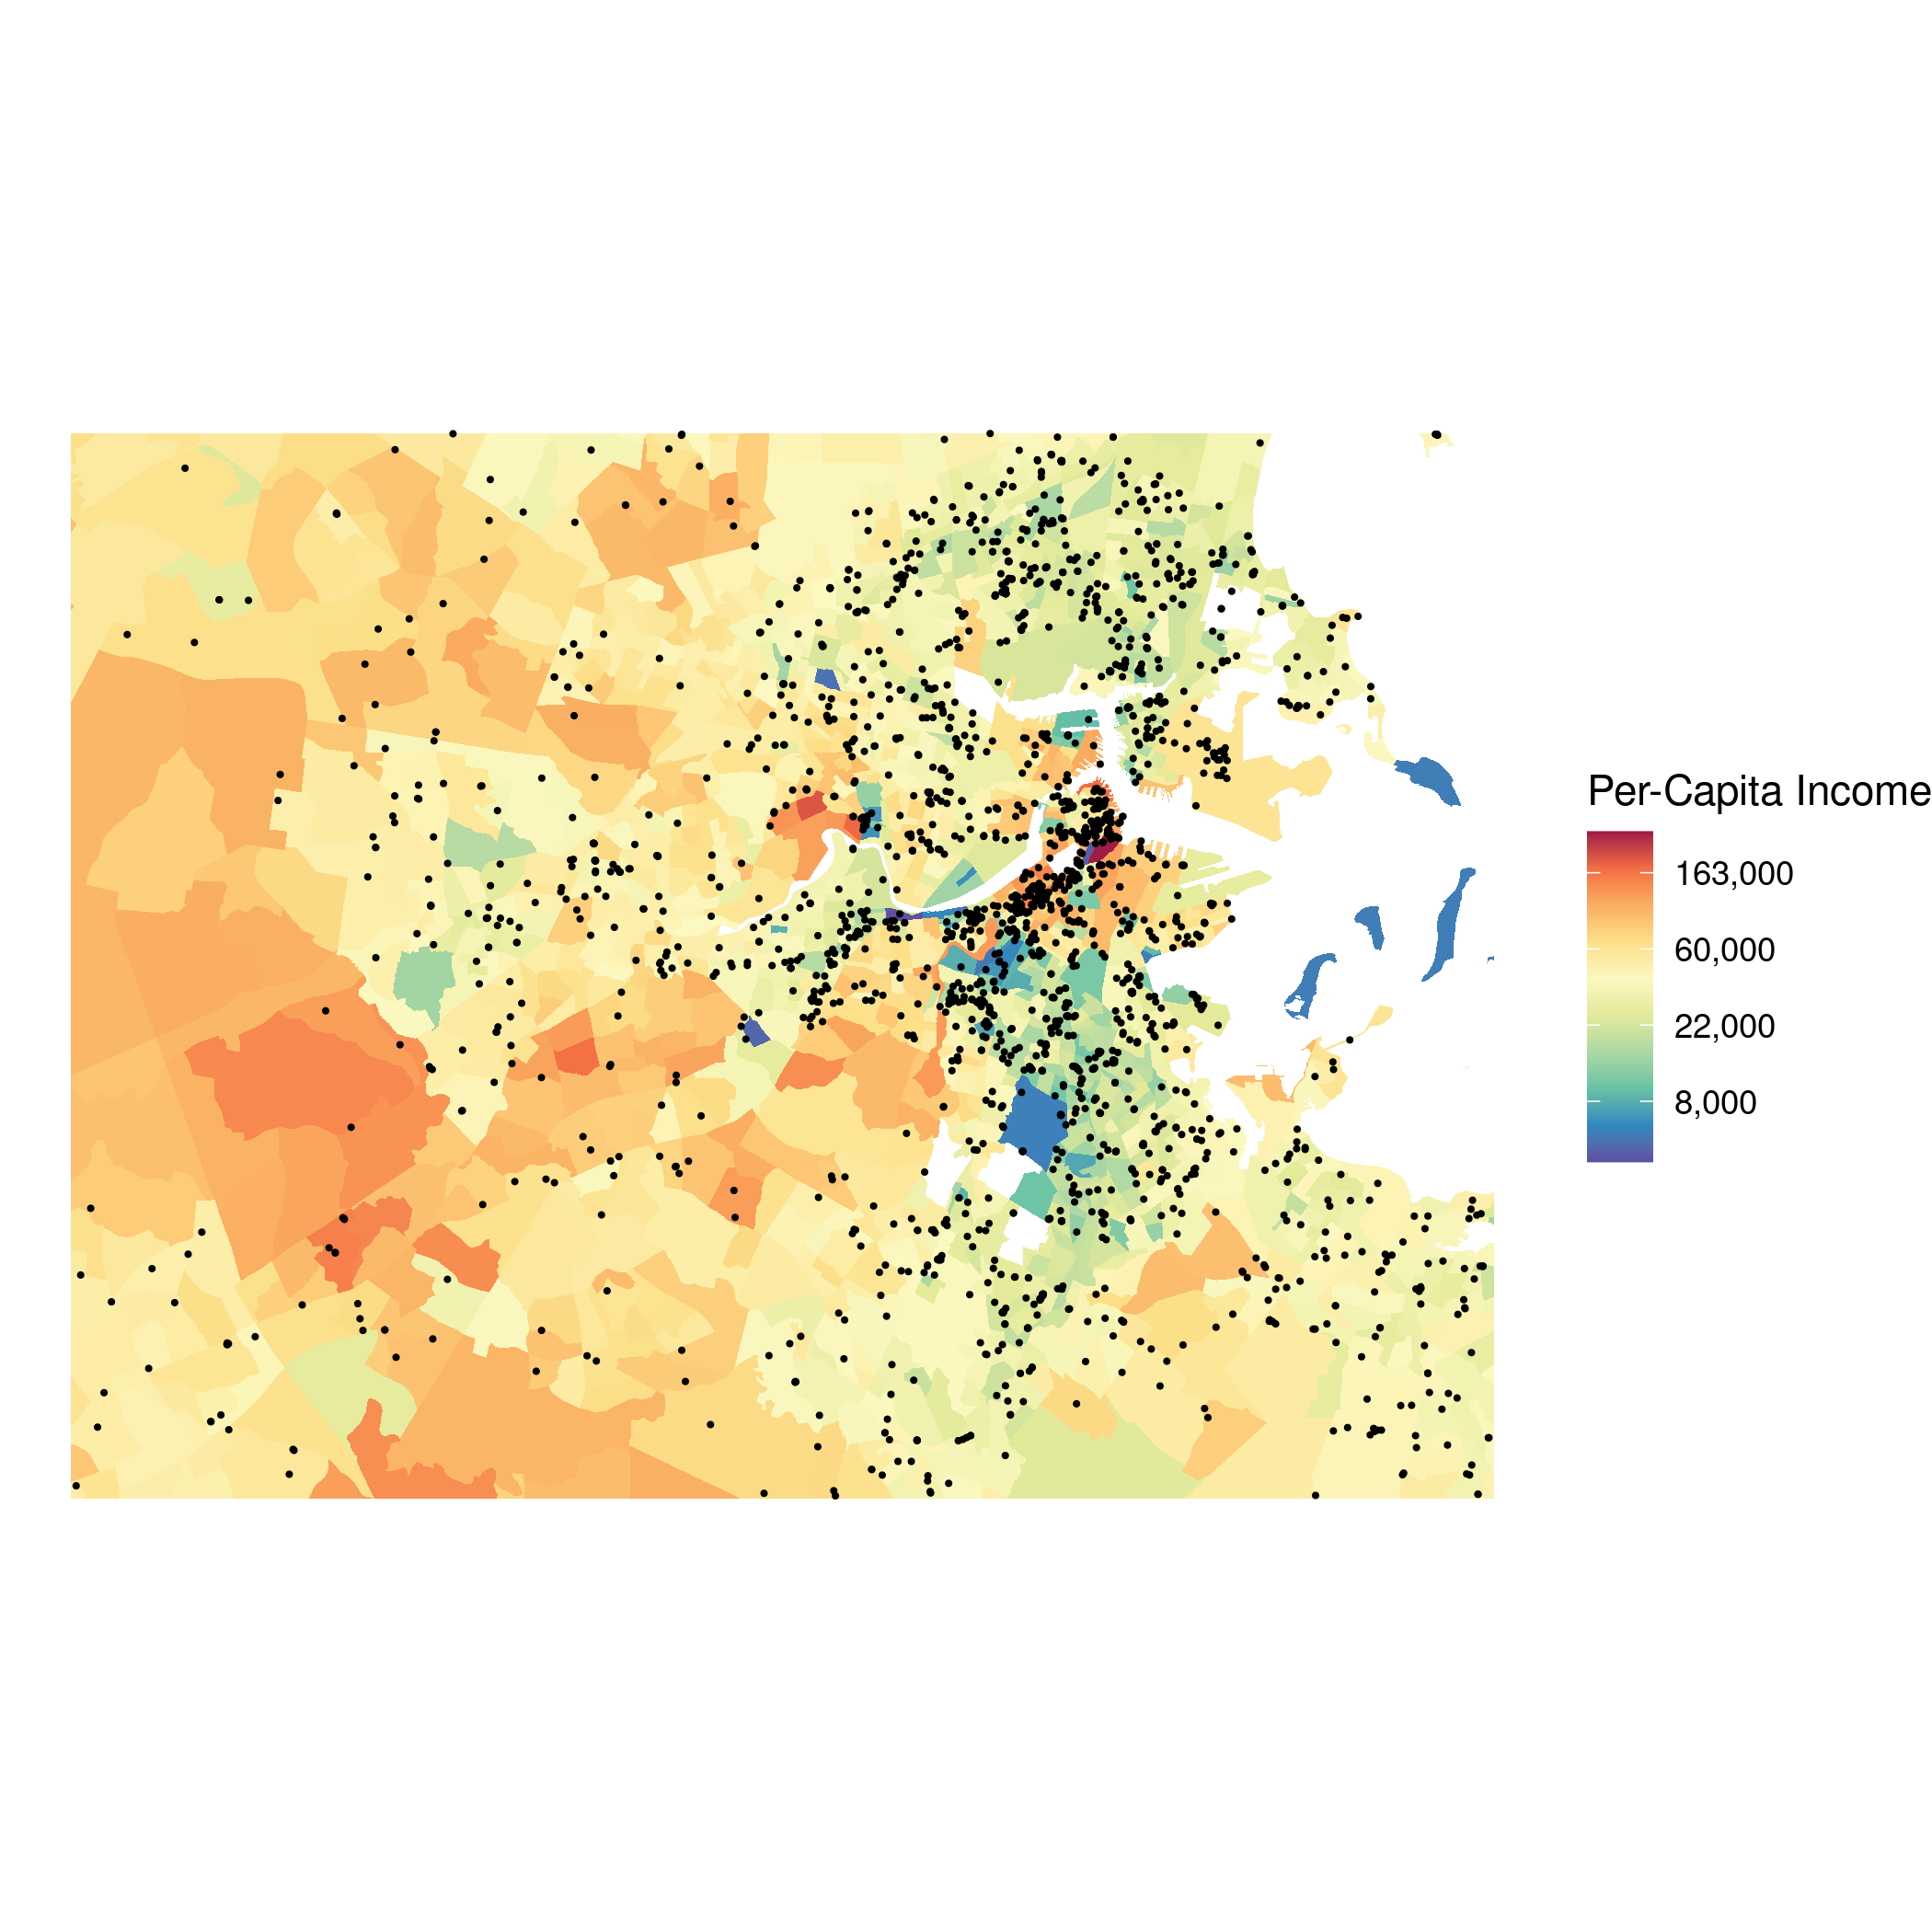
\includegraphics[width=\linewidth]{../res/Boston_Map.png}
  \caption{Here is a map of all tweets in boston, overlaid with income by census block}
  \label{fig:timeseries}
\end{figure}

\section{Methods}
\subsection{Text Data}
Text data used for this project come from Twitter via the University of Vermont’s (UVM) agreement with Twitter to access its streaming API - colloquially referred to as the Decahose - which provides public access to a random 10\% of all public messages on Twitter. The UVM special agreement with Twitter allows for access to this data for research and analysis purposes and we have complied with all the terms of service for Twitter and UVM. 
The Twitter data consists of publicly posted messages, or Tweets, that are short status messages users post to the platform. We used all geolocated Tweets from the Decahose for the period 2012-2016 with a bounding box polygon filter for India, Western Europe and the United States of America. We only considered users’ original content, thus did not include retweets in our analysis.

\subsection{Weather}
We used data on local weather conditions from the North American Land Data Assimilation System (NLDAS), a gridded product developed by several collaborative institutions, including NOAA, NASA, Princeton University, and the University of Washington \href{https://agupubs.onlinelibrary.wiley.com/doi/full/10.1029/2011JD016048}{link}.  This dataset is available at an hourly temporal resolution, and at 1/8th decimal degree spatial resolution \cite{xia_continental-scale_2012}.  We extracted the data for the exact hour and location of each tweet using Google Earth Engine. We extracted several variables from the NLDAS-2 dataset, including temperature, specific humidity, air pressure, total precipitation, and shortwave radiation.  Using temperature, specific humidity, and pressure, we derived relative humidity using methods described by  \cite{bolton_computation_1980}. Then, based on the Heat Index algorithm developed by Steadman \cite{steadman_assessment_1979} and improved upon by Rothfusz and the National Weather service \cite{rothfusz_heat_1990}, we calculated the Heat Index using temperature and relative humidity \cite{heo_comparison_2019}.

ISSUES: deciduous trees lose leaves every year and may not provide much shade cover and heat relief during particular periods of the year when they are leafless.

\subsection{Income}
We used data from the US Census at the Census Block level to estimate the 

\subsection{Land Cover}
To estimate land cover categories and the percentage of tree cover and impervious surfaces, we used data from the National Land Cover Database (NLCD) from the USGS' 2011  \cite{homer_completion_2015} and 2016 \cite{yang_new_2018} landcover datasets. These datasets are national land cover dataset prepared by the Multi-Resolution Land Characteristics (MRLC) Consortium.  These data are at the thirty meter resolution, and provide estimates of the fraction of tree cover and impervious surfaces.  We then associated each tweet with the land cover fraction for the nearest available year and pixel using the geolocation associated with each tweet, extracting landcover values from whichever land cover dataset year was closest in time to the date timestamp of each tweet. We used tree cover as a proxy for amount of potential shade and heat relief in a particular area and can be broadly indicative of generalized wealth. We use impervious surface cover as a proxy for relative proximity to potential natural shade and heat relief, and because individuals in urban environments may be exposed to the urban heat island effect. [NEED SOME CITATIONS HERE] 

\subsection{Sentiment}
We assessed the sentiment expressed in text using several of the most commonly used measures of sentiment. Each of the measures uses validated dictionaries of words that have been assigned positive and negative scores and compares these words with words in the text corpora of interest. For measures of sentiment, we used the Hedonometer \href{https://hedonometer.org/timeseries/en_all/}{(link)}, Afinn \href{http://corpustext.com/reference/sentiment_afinn.html}{(link)}, Textblob \href{https://textblob.readthedocs.io/en/dev/}{(link)}, Vader , SentiwordNet and LIWC tools. These tools assign positive and negative scores to words, then average the scores for each text string. Our text data was multilingual, which can present challenges with analyzing text (cite). Given our interest only in the collection of words used (in aggregate) and not the sequence or nuance of the phrases, we translated all languages into English using Google Translate API and the Microsoft Azure API cognitive services (translator text API) before conducting the sentiment analyses.

Some papers we might cite in this section (only for multilingual work): Vilares et al. 2017 , Lo et al. 2017, Dashtipour et al. 2016.

Discuss issues with text data (gtp) - that it doesn’t capture emoticons, code switching (e.g., [good job! \#fail]), etc.

Issues with sample population (non-representative)

Issues with what people say on social media being attenuated or mismatched from actual emotional state

\subsubsection{Hedonometer}
The Hedonometer \cite{dodds_temporal_2011} is a corpus-based technique to get sentiment score from multi-lingual texts. The core steps are (1) building human evaluations of the happiness of a set of individual words, and (2)using a naive algorithm for scaling up from individual words to texts. For the English corpus, Dodds and others \cite{dodds_temporal_2011} collect 10,222 unique words and used crowd-sourcing platform Amazon Mechanical Turk to get human evaluation of happiness degree for each word in an integer scale from 1 to 9, representing a sad to happy spectrum. Score 5 represents neutral words. Each word will be calculated average score and then the word and happiness score are compiled into a dataset (labMT 1.0). Some illustrative example of words are: 

\[h_{avg} (\text{laughter}) = 8.50 \]
\[h_{avg} (\text{the}) = 4.98\]
\[h_{avg} (\text{hate}) = 2.34\]

The sentiment score for single text will be the mean happiness score for all words in the text.


\subsubsection{VADER}
The VADER sentiment corpus was proposed by Gilbert and Hutto \cite{gilbert_vader_2014} and stands for 'Valence Aware Dictionary for sentiment Reasoning'. It is is a lexicon and rule-based sentiment analysis tool that is specifically attuned to sentiments expressed in social media by incorporating lexical features common to sentiment expression in microblogs

\subsection{Analytic Approach}
To assess whether temperature affects sentiment, we ran a linear regression model that included meteorological measures and sentiment. Independent variables included maximum daily temperature, precipitation and heat index. We also included fixed effects indicator variables at the year-month and decimal degree levels to account for potential biases in unobserved characteristics associated with seasonality and date. We examined the relationships between meteorological variables and sentiment using linear regression models.

\subsection{Data Processing}
We analyzed meteorological data using the R statistics open-source program version 3.6.2  (R Core Team 2019) using R Studio version 1.2.1335 (RStudio Team, 2019) and the raster \href{https://www.rdocumentation.org/packages/raster/versions/3.3-13}{(link)}, sp \href{https://cran.r-project.org/web/packages/sp/index.html}{(link)}, sf \href{https://cran.r-project.org/web/packages/sf/index.html}{(link)}, and stars \href{https://cran.r-project.org/web/packages/stars/index.html}{(link)} processing and geospatial packages installed. Sentiment data was analyzed using python version x.x.x with pandas \href{https://pandas.pydata.org/}{(link)} and numpy \href{https://numpy.org/}{(link)} packages installed. We extracted meteorological data using the geolocated coordinates from the Twitter posts (latitude and longitude). We calculated mean climatological scores (z-scores)using baseline meteorological data from 1990 to present, calculated at a quarter degree resolution, and based on the long-term averages and standard deviation. We calculated z-scores for each day and the overall annual average z-score. For text data cleaning we used the python package tweet-preprocessor \href{https://pypi.org/project/tweet-preprocessor/}{(link)} to remove all text and characters not part of the main text phrase (e.g., URLs, mentions, GIFs, etc.). We converted all dates and times to UTC format.

\section{Results}
(sub-section) DESCRIPTIVE STATISTICS

\begin{figure}[H]
  \centering
  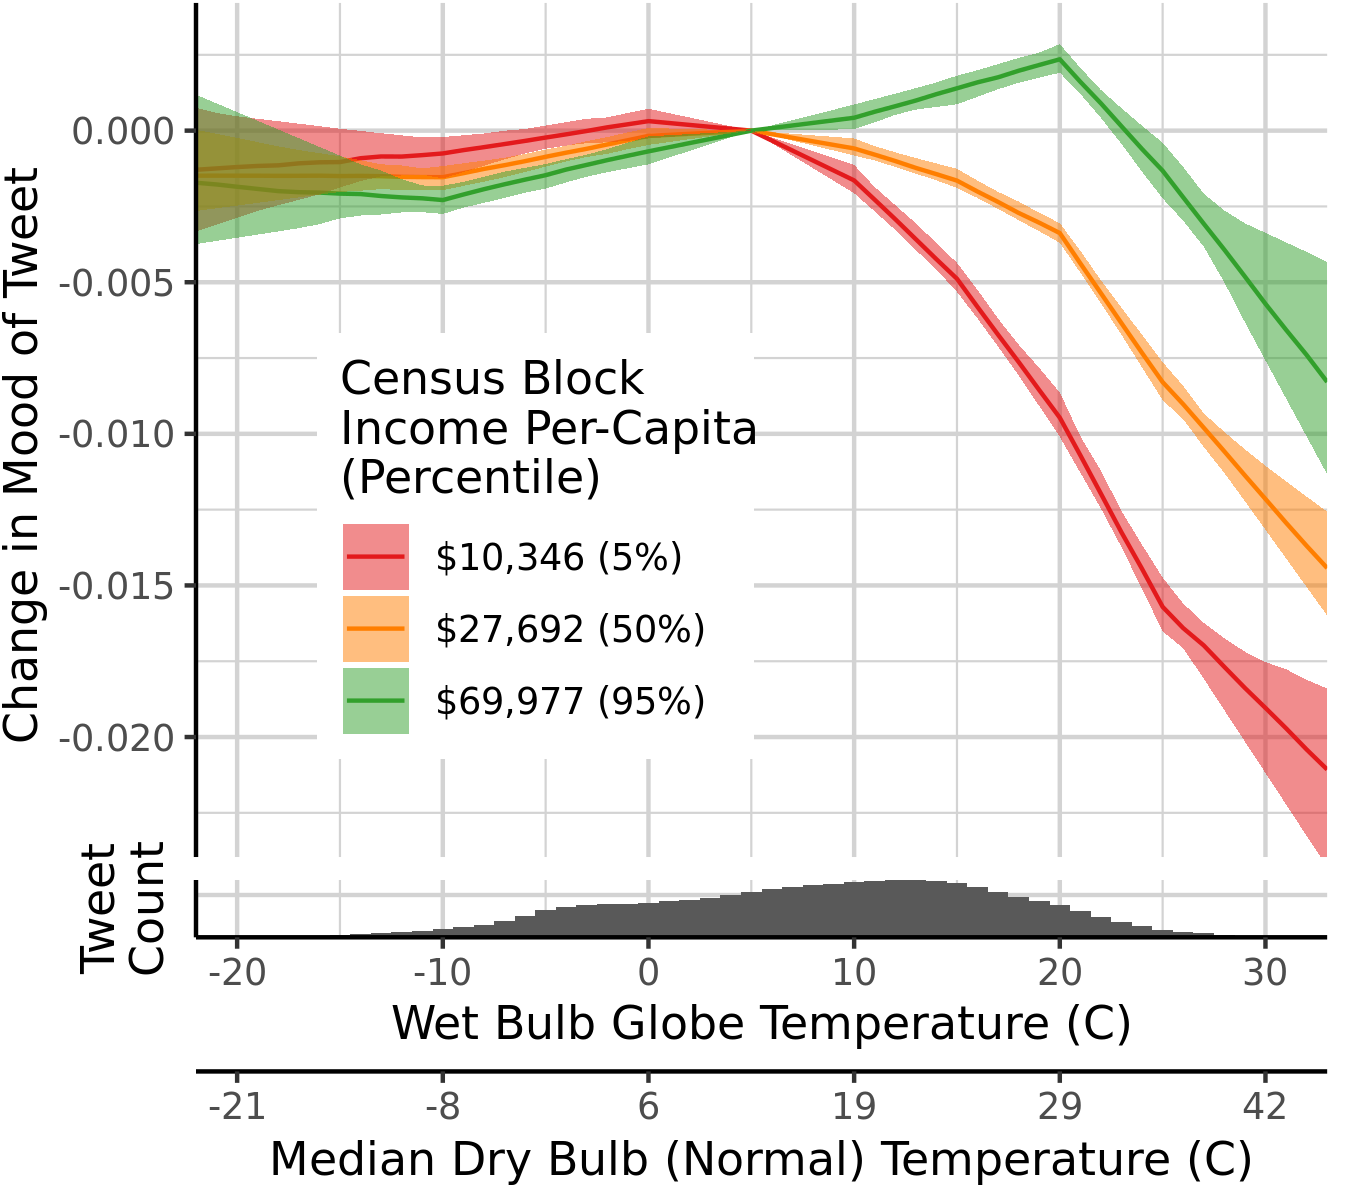
\includegraphics[width=\linewidth]{../res/wbgt-income.png}
  \caption{Change in sentiment across census block income groups as the Wet Bulb Globe Temperature increases.  For census blocks at the 5th percentile for income, even mild temperatures are associated with decreases in mood, while at higher temperatures, sentiment continues to decline.  For high-income census blocks at the 95th percentile, on the other hand, temperature must be quite high before a decrease in sentiment is observed.}
  \label{fig:wbgt-income}
\end{figure}



Figure of heatmap of tweet density across USA (pick a year? entire dataset of georeferenced tweets?)

(sub-section) TEMPERATURE and HUMIDITY
Figure of distribution of max and min temperatures
Comment from Patrick Baylis on our "preliminary results". 2nd comment from Patrick

(sub-section) INCOME

(sub-section?) SENTIMENT
Figure of distribution of observed sentiment scores (by Hedonometer, Vader, etc.)

Comment from Patrick Baylis on our "preliminary results" doc


\section{Discussion}

\section{Conclusion}

\section{Acknowledgements}
For funding, advising, SESYNC grant number?, etc.

\printbibliography

\section*{Supplemental Info}
\setcounter{table}{0}
\setcounter{figure}{0}
\setcounter{section}{0}
\renewcommand{\thetable}{S\arabic{table}}
\renewcommand{\thefigure}{S\arabic{figure}}
\renewcommand{\thesection}{S\arabic{section}}

\section*{Text Snippets Not Used Here but We Might Want to Keep}
Gaps on above we intend to fill in:
Our research aim and objectives
Its contribution

From Intro/Background
Changes in climate result in fluctuations in the frequency, intensity, spatial extent, duration, and timing of weather resulting in unprecedented climate extremes . Changing climate is putting pressures on environmental and social system health and necessitating changes in how we respond to environmental conditions and anticipate (and plan for) future conditions. (cite IPCC report on health and environment, also cite the Lancet report on climate and health). 

[from our Jan/Feb 2020 draft working manuscript in Google Docs]
Climate change is a universal issue as it affects every country in the world. Changes in climate result in fluctuations in the frequency, intensity, spatial extent, duration, and timing of weather resulting in unprecedented climate extremes \href{https://www.ipcc.ch/site/assets/uploads/2018/03/SREX-Chap3_FINAL-1.pdf}{(link)}. Changing climate is putting pressures on environmental and social system health and necessitating changes in how we respond to environmental conditions and anticipate (and plan for) future conditions. (cite IPCC report on health and environment, also cite the Lancet report on climate and health).

Dehghan et al. 2012  The evaluation of heat stress through monitoring environmental factors and physiological responses in melting and casting industries workers. High prevalence of industrial workers experiencing heat stress. Relatively low humidity conditions made it necessary to alter their work/rest cycles. \href{http://www.ijehe.org/article.asp?issn=2277-9183;year=2012;volume=1;issue=1;spage=21;epage=21;aulast=Dehghan}{link}

?. (from intro) Increased variability around environmental norms (e.g., lower/higher temperatures, changes in timing, magnitude, duration of precipitation or dry spells, etc.) can amplify the effects on systems. Increased uncertainty in planning for these events and ability to respond to them (adaptive capacity). - draw in cultural risk and social practice theories, here?

NOTES: Scaling back out → we are exploring temperature and sentiment (in Tweets) across languages. This is a clear innovation that builds on the existing work from the Baylis et al. team (in their plosONE paper) and in fact is something they recommended be done - recommended to us as a team, too.

We know that temps affect sentiment, but (1) Is this effect observable across languages? (2) Is this effect moderated by factors like wealth?

We could ask similar questions substituting in the patent filings, too (sub-project 3 in our previous work-plan). These questions - and likely the methods used to answer these questions - are quite portable and compelling and may take the form for the patent work like this: Given we know that temperature affects worker productivity (increased temp increases productivity up to 13C, sharp negative decline thereafter), can we observe this pattern in patent filings? Across various geographies? Are there lags in filings after unusually cold or hot temperature events?

For the Twitter data, using text translated into a base language is fully appropriate and a frequently used method if looking for latent text structures in topic modeling (see Proksch et al. 2018 for an alternative). For sentiment analysis on multilingual datasets, we'll need to decide on an approach (see Ling Lo et al. 2016 review) but there are several that are good. If we wanted to use another open-source option, we could follow that laid out by Lucas and others (2015).

Proskch et al. 2018 paper --> \href{https://onlinelibrary.wiley.com/doi/full/10.1111/lsq.12218}{link} 

Ling Lo et al. 2016 paper --> \href{https://link.springer.com/article/10.1007/s10462-016-9508-4}{link} 

Lucas et al. 2015 paper --> \href{https://www.cambridge.org/core/journals/political-analysis/article/computerassisted-text-analysis-for-comparative-politics/CC8B2CF63A8CC36FE00A13F9839F92BB}{link}
 





\end{document}
